% IEEE Design & Test feature article, laid out after the D&T house pattern
% (department tag, sans-serif title and headings, unnumbered sentence-case
% sections, small-caps lead-in, unheaded closing with end mark, "References"
% and bios without heading, "Direct questions" line). CEDA author guidelines
% take precedence: <= 5,000 words incl. references and bios (200 per figure or
% table), <= 12 references, title <= 9 words, introduction 1-5 paragraphs,
% conclusion 1-2 paragraphs, bios with position, degree, <= 3 interests, e-mail.
% Author manuscript for IEEE Design & Test (SI: SBCCI 2026). D&T publishes no
% template; production applies the magazine layout after acceptance. This file
% follows the CEDA author guidelines (<= 5,000 words incl. references and bios,
% 200 per figure/table; <= 12 references; title <= 9 words; opening 1-5
% paragraphs without an "Introduction" heading; conclusion 1-2 paragraphs;
% bios with position, degree, <= 3 interests, e-mail) and the structure of
% published D&T features (unnumbered sentence-case headings).
\documentclass[10pt,twocolumn]{article}
\usepackage[utf8]{inputenc}
\usepackage[T1]{fontenc}
\usepackage{mathptmx}
\usepackage[letterpaper,top=0.75in,bottom=0.85in,left=0.7in,right=0.7in,columnsep=0.24in]{geometry}
\usepackage{graphicx,booktabs,amsmath,xcolor,array,cite,url,textcomp}
\usepackage[shortlabels]{enumitem}
\graphicspath{{figures/}}
\usepackage[font=footnotesize,labelfont=bf,labelsep=period,skip=4pt]{caption}
\usepackage{titlesec,fancyhdr}
\setcounter{secnumdepth}{0}
\titleformat{\section}{\normalfont\large\bfseries\color{black!80}}{}{0pt}{}
\titlespacing*{\section}{0pt}{9pt plus 2pt}{3pt}
\renewcommand{\figurename}{Figure}
\renewcommand{\tablename}{Table}
\captionsetup[table]{position=top}
\pagestyle{fancy}\fancyhf{}
\fancyhead[L]{\footnotesize\itshape IEEE Design \& Test --- Special Issue: SBCCI 2026}
\fancyhead[R]{\footnotesize\itshape Alencar et al.: Burn-In Thermal Control Sets What Aging Sensors Can See}
\fancyfoot[C]{\footnotesize\thepage}
\renewcommand{\headrulewidth}{0.3pt}
\setlength{\parskip}{0pt}
\setlist{itemsep=1pt,parsep=0pt}
\definecolor{pid}{HTML}{1F5FBF}\definecolor{bb}{HTML}{D9661F}
\newcommand{\Tmin}{T_{\min}}
\newcommand{\tint}{\tau_{\mathrm{int}}}
% units without siunitx (keeps the source buildable on TeX Live 2020)
\newcommand{\degC}{\,\textdegree C}
\newcommand{\unit}[1]{\,\mathrm{#1}}
\newcommand{\mcnth}{\,m\,cnt/h}
\newcommand{\dttitle}{Burn-In Thermal Control Sets What Aging Sensors Can See}
\hyphenation{Arrhe-nius}
% every result printed below comes from analysis/ through these macros
% AUTO-GENERATED by analysis/derive.py -- do not edit by hand.
% Every number printed in the manuscript comes from one of these macros.
\newcommand{\vAFBB}{31.1}
\newcommand{\vAFBBlong}{31.8}
\newcommand{\vAFPID}{51.3}
\newcommand{\vAFRCA}{78.1}
\newcommand{\vAFdevBB}{$-$33}
\newcommand{\vAFdevPID}{12}
\newcommand{\vAFfullBB}{31.1}
\newcommand{\vAFfullPID}{51.3}
\newcommand{\vAFratio}{1.65}
\newcommand{\vAFratioFull}{1.65}
\newcommand{\vAFratioFullHi}{1.90}
\newcommand{\vAFratioFullLo}{1.43}
\newcommand{\vAFratioHi}{1.90}
\newcommand{\vAFratioHiOne}{1.9}
\newcommand{\vAFratioLo}{1.43}
\newcommand{\vAFratioLoOne}{1.4}
\newcommand{\vAFratioMeanOnly}{1.66}
\newcommand{\vBBlongLrvEight}{530}
\newcommand{\vBBlongSigRatio}{0.99}
\newcommand{\vBetaBB}{$-$7.4}
\newcommand{\vBetaBBlong}{$-$6.0}
\newcommand{\vBetaHiBB}{$-$3.9}
\newcommand{\vBetaHiBBlong}{$-$4.6}
\newcommand{\vBetaHiPID}{$-$16.3}
\newcommand{\vBetaHiRCA}{$-$14.4}
\newcommand{\vBetaLoBB}{$-$11.2}
\newcommand{\vBetaLoBBlong}{$-$7.5}
\newcommand{\vBetaLoPID}{$-$45.5}
\newcommand{\vBetaLoRCA}{$-$22.1}
\newcommand{\vBetaPID}{$-$30.6}
\newcommand{\vBetaRCA}{$-$18.3}
\newcommand{\vCadBB}{2}
\newcommand{\vCadBBlong}{2}
\newcommand{\vCadPID}{1}
\newcommand{\vCadRCA}{1}
\newcommand{\vCbbBound}{0.91}
\newcommand{\vCbbLrv}{0.02}
\newcommand{\vCpidBound}{1.00}
\newcommand{\vCpidHour}{0.00}
\newcommand{\vCpidLrv}{0.12}
\newcommand{\vDeltaFive}{0.9}
\newcommand{\vDeltaTen}{1.8}
\newcommand{\vDeltaTwenty}{3.4}
\newcommand{\vDtdtGainPct}{0.6}
\newcommand{\vDurBB}{23.1}
\newcommand{\vDurBBlong}{164.2}
\newcommand{\vDurPID}{23.1}
\newcommand{\vDurPair}{23.08}
\newcommand{\vDurPairPost}{22}
\newcommand{\vDurPostBB}{22.1}
\newcommand{\vDurPostBBlong}{163.2}
\newcommand{\vDurPostPID}{22.1}
\newcommand{\vDurPostRCA}{213.6}
\newcommand{\vDurRCA}{214.6}
\newcommand{\vEmaxSimc}{4.5}
\newcommand{\vEmaxThermo}{7.0}
\newcommand{\vEmaxTuned}{1.9}
\newcommand{\vEqhBB}{711}
\newcommand{\vEqhBBlong}{5{,}175}
\newcommand{\vEqhMeanOnlyBB}{711}
\newcommand{\vEqhMeanOnlyPID}{1{,}182}
\newcommand{\vEqhPID}{1{,}182}
\newcommand{\vEqhRCA}{16{,}701}
\newcommand{\vEqhTrajBB}{717}
\newcommand{\vEqhTrajPID}{1{,}184}
\newcommand{\vFinalKd}{5.0}
\newcommand{\vFinalKiE}{1.06}
\newcommand{\vFinalKp}{2.78}
\newcommand{\vFopdtK}{1.56}
\newcommand{\vFopdtRmse}{5.1}
\newcommand{\vFopdtTau}{1307.2}
\newcommand{\vFopdtTfinal}{103.2}
\newcommand{\vFopdtTheta}{150.6}
\newcommand{\vFopdtTmax}{106.9}
\newcommand{\vFopdtTzero}{25.21}
\newcommand{\vHSBB}{3.50}
\newcommand{\vHSBBlong}{3.62}
\newcommand{\vHSPID}{2.18}
\newcommand{\vHSRCA}{3.43}
\newcommand{\vHystBB}{0.11}
\newcommand{\vHystBBlong}{0.05}
\newcommand{\vHystPID}{0.01}
\newcommand{\vHystPct}{12}
\newcommand{\vHystRCA}{0.02}
\newcommand{\vJensen}{1.1}
\newcommand{\vLagBB}{2}
\newcommand{\vLagBBlong}{4}
\newcommand{\vLagPID}{$-$2}
\newcommand{\vLagRCA}{0}
\newcommand{\vLateHiBB}{$-$1.2}
\newcommand{\vLateHiPID}{$-$2.8}
\newcommand{\vLateLoBB}{$-$11.8}
\newcommand{\vLateLoPID}{$-$7.7}
\newcommand{\vLateSlopeBB}{$-$6.5}
\newcommand{\vLateSlopePID}{$-$5.3}
\newcommand{\vLrvBB}{14}
\newcommand{\vLrvBBlong}{77}
\newcommand{\vLrvPID}{59}
\newcommand{\vLrvRCA}{1{,}482}
\newcommand{\vMIdtBB}{1.60}
\newcommand{\vMIdtBBlong}{1.65}
\newcommand{\vMIdtPID}{0.78}
\newcommand{\vMIdtRCA}{0.60}
\newcommand{\vMIexcessBB}{0.07}
\newcommand{\vMIexcessBBlong}{0.06}
\newcommand{\vMIrawBB}{1.70}
\newcommand{\vMIrawBBlong}{1.74}
\newcommand{\vMIrawPID}{0.64}
\newcommand{\vMIrawRCA}{1.13}
\newcommand{\vMIresBB}{0.100}
\newcommand{\vMIresBBlong}{0.071}
\newcommand{\vMIresPID}{0.335}
\newcommand{\vMIresQBB}{0.031}
\newcommand{\vMIresQBBlong}{0.016}
\newcommand{\vMIresQPID}{0.693}
\newcommand{\vMIresQRCA}{0.009}
\newcommand{\vMIresRCA}{0.089}
\newcommand{\vMeanShare}{102}
\newcommand{\vNLaw}{0.32}
\newcommand{\vNpostBB}{39{,}700}
\newcommand{\vNpostBBlong}{293{,}440}
\newcommand{\vNpostPID}{79{,}486}
\newcommand{\vNpostRCA}{768{,}878}
\newcommand{\vNrawBB}{41{,}499}
\newcommand{\vNrawBBlong}{295{,}239}
\newcommand{\vNrawPID}{83{,}086}
\newcommand{\vNrawRCA}{772{,}484}
\newcommand{\vOverSimc}{6.5}
\newcommand{\vOverThermo}{8.1}
\newcommand{\vOverTuned}{0.7}
\newcommand{\vPIDspMax}{83}
\newcommand{\vPIDspMin}{83}
\newcommand{\vPenHigh}{1.69}
\newcommand{\vPenLow}{1.29}
\newcommand{\vPenMid}{1.62}
\newcommand{\vPenMidHi}{1.77}
\newcommand{\vPenMidLo}{1.47}
\newcommand{\vPenNoise}{1.16}
\newcommand{\vPenNoiseSigOnly}{1.16}
\newcommand{\vPenStress}{1.40}
\newcommand{\vPenStressPow}{1.11}
\newcommand{\vPerrBbBound}{1.1}
\newcommand{\vPerrBbLrv}{41}
\newcommand{\vPerrPidBound}{0.0}
\newcommand{\vPerrPidLrv}{30}
\newcommand{\vPowNBB}{1.50}
\newcommand{\vPowNBBlong}{0.24}
\newcommand{\vPowNPID}{0.05}
\newcommand{\vPowNRCA}{0.32}
\newcommand{\vPowNblockRCA}{0.35}
\newcommand{\vPsINV}{19.84}
\newcommand{\vPsRCA}{17.86}
\newcommand{\vPtpSimc}{7.2}
\newcommand{\vPtpThermo}{10.5}
\newcommand{\vPtpTuned}{1.8}
\newcommand{\vRCAMIksg}{1.18}
\newcommand{\vRCAMIrawCIhi}{1.17}
\newcommand{\vRCAMIrawCIlo}{1.09}
\newcommand{\vRCAMIrawHi}{1.17}
\newcommand{\vRCAMIrawLo}{1.09}
\newcommand{\vRCAMIremoved}{85}
\newcommand{\vRCATmax}{134}
\newcommand{\vRCATmin}{117}
\newcommand{\vRCAbayes}{$-$18.1}
\newcommand{\vRCAbayesHi}{$-$17.7}
\newcommand{\vRCAbayesLo}{$-$18.5}
\newcommand{\vRCAcorrStCorr}{$-$0.73}
\newcommand{\vRCAcorrStRaw}{$-$0.35}
\newcommand{\vRCAcrlb}{0.17}
\newcommand{\vRCAcurrSlope}{0.041}
\newcommand{\vRCAdriftCnt}{3.9}
\newcommand{\vRCAdriftPs}{70}
\newcommand{\vRCAfirstHalf}{$-$28.3}
\newcommand{\vRCAfirstSigRatio}{1.01}
\newcommand{\vRCAfloor}{0.5}
\newcommand{\vRCAlrvEight}{7{,}793}
\newcommand{\vRCAlrvGrowth}{17}
\newcommand{\vRCAlrvQuarter}{464}
\newcommand{\vRCAlrvWhite}{82}
\newcommand{\vRCAneff}{6{,}591}
\newcommand{\vRCAneffSeq}{6{,}591}
\newcommand{\vRCAnull}{0.10}
\newcommand{\vRCAoven}{93.9}
\newcommand{\vRCAovenMax}{103.6}
\newcommand{\vRCAovenMin}{89.5}
\newcommand{\vRCAovensd}{1.8}
\newcommand{\vRCAsecondHalf}{$-$14.8}
\newcommand{\vRCAspChanges}{49}
\newcommand{\vRCAspMax}{99}
\newcommand{\vRCAspMin}{91}
\newcommand{\vRippleBB}{1.0}
\newcommand{\vRippleBBlong}{1.0}
\newcommand{\vRipplePID}{0.2}
\newcommand{\vRipplePostBB}{1.0}
\newcommand{\vRipplePostPID}{0.1}
\newcommand{\vRippleRCA}{0.4}
\newcommand{\vRsqBB}{92.1}
\newcommand{\vRsqBBlong}{92.5}
\newcommand{\vRsqPID}{59.2}
\newcommand{\vRsqRCA}{73.8}
\newcommand{\vRsqTBB}{92.1}
\newcommand{\vRsqTBBlong}{92.5}
\newcommand{\vRsqTPID}{54.5}
\newcommand{\vRsqTRCA}{73.8}
\newcommand{\vSPjumpFrac}{12}
\newcommand{\vSPjumpN}{48}
\newcommand{\vSdRatioThermo}{8.9}
\newcommand{\vSdSimc}{1.94}
\newcommand{\vSdThermo}{3.38}
\newcommand{\vSdTuned}{0.38}
\newcommand{\vSeqZbb}{3.1}
\newcommand{\vSeqZpid}{6.5}
\newcommand{\vSigBB}{0.90}
\newcommand{\vSigBBlong}{0.89}
\newcommand{\vSigCBB}{0.78}
\newcommand{\vSigCBBlong}{0.72}
\newcommand{\vSigCPID}{1.61}
\newcommand{\vSigCRCA}{0.57}
\newcommand{\vSigPID}{0.69}
\newcommand{\vSigRCA}{0.84}
\newcommand{\vSigRatio}{1.31}
\newcommand{\vSigRatioPct}{31}
\newcommand{\vSigRawBB}{0.90}
\newcommand{\vSigRawBBlong}{0.95}
\newcommand{\vSigRawPID}{0.73}
\newcommand{\vSigRawRCA}{1.55}
\newcommand{\vSigRawRatio}{1.24}
\newcommand{\vSigRawRatioCommon}{1.24}
\newcommand{\vSigRawRatioPct}{24}
\newcommand{\vSigRevRatio}{1.31}
\newcommand{\vSigRevRatioPct}{31}
\newcommand{\vSimcKiE}{2.31}
\newcommand{\vSimcKp}{2.78}
\newcommand{\vTBB}{107.73}
\newcommand{\vTBBlong}{108.15}
\newcommand{\vTPID}{117.04}
\newcommand{\vTRCA}{125.05}
\newcommand{\vTauBB}{1}
\newcommand{\vTauBBlong}{1}
\newcommand{\vTauBBs}{1.3}
\newcommand{\vTauBBsamp}{0.7}
\newcommand{\vTauPID}{0}
\newcommand{\vTauPIDs}{1.2}
\newcommand{\vTauPIDsamp}{0.6}
\newcommand{\vTauRCA}{58}
\newcommand{\vTauRatio}{1.15}
\newcommand{\vTauTipBB}{148}
\newcommand{\vTauTipBBlong}{154}
\newcommand{\vTauTipPID}{169}
\newcommand{\vTauTipRCA}{314}
\newcommand{\vTerrBB}{$-$7.27}
\newcommand{\vTerrBBlong}{$-$6.85}
\newcommand{\vTerrFullBB}{$-$7.27}
\newcommand{\vTerrFullPID}{2.04}
\newcommand{\vTerrPID}{2.04}
\newcommand{\vTerrRCA}{0.05}
\newcommand{\vTfullBB}{107.73}
\newcommand{\vTfullPID}{117.04}
\newcommand{\vTminBBBound}{32}
\newcommand{\vTminBBBoundHi}{33}
\newcommand{\vTminBBBoundLo}{25}
\newcommand{\vTminBBLrv}{144}
\newcommand{\vTminBBLrvHi}{151}
\newcommand{\vTminBBLrvLo}{114}
\newcommand{\vTminBBSeq}{26}
\newcommand{\vTminBBSeqHi}{27}
\newcommand{\vTminBBSeqLo}{21}
\newcommand{\vTminBound}{20}
\newcommand{\vTminLrv}{89}
\newcommand{\vTminSeq}{16}
\newcommand{\vTminSeqBBlong}{14}
\newcommand{\vTminTip}{34}
\newcommand{\vTminTipCorr}{27}
\newcommand{\vTpostBB}{107.76}
\newcommand{\vTpostPID}{117.13}
\newcommand{\vTsdBB}{2.64}
\newcommand{\vTsdBBlong}{2.71}
\newcommand{\vTsdFullBB}{2.64}
\newcommand{\vTsdFullPID}{1.25}
\newcommand{\vTsdPID}{1.25}
\newcommand{\vTsdPostBB}{2.63}
\newcommand{\vTsdPostPID}{0.93}
\newcommand{\vTsdRCA}{1.83}
\newcommand{\vTsdRatio}{2.1}
\newcommand{\vTsdRatioFull}{2.1}
\newcommand{\vVmeanBB}{1.2988}
\newcommand{\vVmeanBBlong}{1.2989}
\newcommand{\vVmeanPID}{1.2967}
\newcommand{\vVmeanRCA}{1.3999}
\newcommand{\vVsdBB}{6.1}
\newcommand{\vVsdBBlong}{6.1}
\newcommand{\vVsdFullBB}{6.1}
\newcommand{\vVsdFullPID}{3.6}
\newcommand{\vVsdPID}{3.6}
\newcommand{\vVsdRCA}{1.3}
\newcommand{\vWbbBound}{30}
\newcommand{\vWbbLrv}{135}
\newcommand{\vWpidBound}{18}
\newcommand{\vWpidLrv}{80}
\newcommand{\vdBICBB}{0}
\newcommand{\vdBICBBlong}{4{,}363}
\newcommand{\vdBICPID}{1{,}902}
\newcommand{\vdBICRCA}{630}
\newcommand{\vdBICblockBBlong}{70}
\newcommand{\vdBICblockRCA}{28}
\newcommand{\vdT}{9.37}
\newcommand{\vdTfull}{9.31}
\newcommand{\vkTBB}{1.15}
\newcommand{\vkTBBlong}{1.23}
\newcommand{\vkTPID}{0.43}
\newcommand{\vkTRCA}{1.47}

\begin{document}

\twocolumn[{%
\begin{center}
{\footnotesize\scshape Feature Article --- Special Issue: SBCCI 2026}\\[6pt]
{\LARGE\bfseries Burn-In Thermal Control Sets What\\[2pt] Aging Sensors Can See}\\[8pt]
{\normalsize Danilo Alencar, Lucas Nogueira, Alisson Barros, Arthur Pamplona, Andre Grangeiro, and Jarbas Silveira}\\
{\small\itshape Laboratory of Electronic Systems and Circuits (LESC), Universidade Federal do Cear\'a, Fortaleza, Brazil}\\[3pt]
{\normalsize Fabian Vargas}\\
{\small\itshape IHP -- Leibniz Institute for High Performance Microelectronics, Frankfurt (Oder), Germany}\\[8pt]
\begin{minipage}{0.86\textwidth}
\small\noindent\textbf{\textit{Abstract}---}On-chip aging sensors validated under burn-in feed silicon lifecycle management (SLM), yet burn-in benches are specified at the chamber, not at the die the sensor sees. On one FPGA and slack sensor, we compare a stock thermostatic oven with a die-referenced PID oven. The thermostat under-delivers Arrhenius acceleration by \vAFratio$\times$, through mean die-temperature shortfall rather than ripple, and leaves \vSigRawRatio$\times$ more residual sensor noise. A \vDurRCA-hour PID campaign resolves a sublinear drift whose detection time depends on slow residual wander, and a thermostatic bench would lengthen it by a projected \vPenLow--\vPenHigh$\times$. We propose a reporting checklist.\\[4pt]
\noindent\textbf{\textit{Keywords}---}Burn-in, on-chip aging sensor, silicon lifecycle management, FPGA, thermal control, acceleration factor, detectability.
\end{minipage}
\end{center}
\vspace{6pt}}]
\renewcommand{\thefootnote}{}\footnotetext{\scriptsize This article extends ``Quantifying the Effect of Burn-In Thermal Control on Delivered Acceleration Factor and On-Chip Slack-Sensor Fidelity in an FPGA Target,'' presented at the 39th Symposium on Integrated Circuits and Systems Design (SBCCI 2026)~\cite{sbcci26}.}\renewcommand{\thefootnote}{\arabic{footnote}}

% ---------------------------------------------------------------
% Opening (no heading in D&T; CEDA: 1-5 paragraphs)
\noindent On-chip aging sensors are moving from research prototypes into the silicon lifecycle management (SLM) stack, where their readings drive adaptive voltage scaling (AVS), remaining-useful-life estimation, and maintenance decisions~\cite{kashyap,niemann}. Before a sensor is trusted in the field, it is usually validated under accelerated burn-in: the device is heated and over-volted, and the sensor is expected to report the resulting delay degradation. FPGA aging sensors have been validated this way for over a decade~\cite{valdes}.

The standards that govern burn-in, JEDEC JESD22-A108~\cite{jedec} and MIL-STD-883 Method~1015~\cite{mil}, set the stress mainly through the \emph{chamber}: ambient temperature, its tolerance, and the applied bias, with junction temperature inferred from them. That a powered device heats itself, so that its junction runs above the chamber, is well known in industrial burn-in; with technology scaling it drove per-device thermal management and junction-temperature control~\cite{vassighi,semenov}. What has not been examined is how this gap affects the \emph{validation of on-chip sensors}, which sample the die rather than the chamber. The question matters because a sensor's own aging already shifts its calibration~\cite{anik}: a validation bench that adds its own, unreported stress and noise makes the sensor's behavior harder to separate from the bench's.

Our SBCCI~2026 paper~\cite{sbcci26} compared a thermostatic (bang-bang) oven and a closed-loop PID oven on the same FPGA and sensor and found that the two benches delivered different stress and different reversible noise. This article asks the practical follow-up: \emph{how long must a burn-in run last before a sensor can see aging, and how much does the bench change that time?} Answering it needs the aging rate the bench induces and the noise it injects, which a 23-hour campaign cannot provide.

The argument is a chain: the bench sets the die-temperature trajectory; its mean fixes the stress delivered and hence the aging signal, its ripple sets the reversible noise, and signal and noise together fix how long a burn-in must run before the sensor sees aging, a limit every SLM function trained on the result inherits. Beyond the conference version, the main contributions of this work are:
\begin{enumerate}
\item \textbf{A source decomposition of the delivered-stress bias.} The \vAFratio$\times$ acceleration-factor gap is set by the mean die-temperature shortfall; thermostat ripple contributes \vRippleBB\%, as a second-order expansion predicts. We translate this into a die-level tracking budget.
\item \textbf{A \vDurRCA-hour sustained-stress campaign}, first reported here, on a second monitored circuit, in which the sensor resolves a sublinear slack drift after PVT correction.
\item \textbf{Detection time, three ways.} A white-noise bound, a long-run-variance estimate, and a sequential test give the burn-in duration needed to see the drift; they differ because the residual wanders slowly and aging is sublinear, and we report all three.
\item \textbf{A measured bench penalty on detectability.} The residual noise and decorrelation of both benches are measured on the paired runs; the aging law that converts delivered acceleration into drift rate is the remaining assumption, and we bracket it.
\item \textbf{A reproducible, commodity PID bench}, documented from plant identification to tuning and validated against the stock thermostat at a second setpoint.
\item \textbf{A five-item reporting checklist} for any 1-Hz burn-in log.
\end{enumerate}

We first describe the instrument, the benches, and the analysis methods, then examine delivered stress, reversible noise, and detectability in turn, and close with the reporting checklist. In short, the bench's mean die temperature, not its ripple, sets the stress; its noise and that stress together set a detection time of \vTminSeq--\vTminLrv\,h on the PID bench, which a thermostatic bench would lengthen.

% ---------------------------------------------------------------
\section{Instrument, benches, and methods}

\textbf{Sensor and DUT.} The DUT is a 28\,nm Xilinx Artix-7 FPGA on a Nexys~4~DDR board; every campaign below ran on the same board. The instrument is our auto-tuning slack sensor~\cite{sbcci25}: an MMCM dynamic phase shift advances a sampling clock in fixed steps until an XOR comparator detects that the monitored path's output has not yet settled, and the number of steps is reported as the path's slack in counts (cnt). The step is $1/(56f_{\mathrm{VCO}})$: 19.85\,ps in the inverter-chain design of the paired runs~\cite{sbcci26} and \vPsRCA\,ps in the bitstream of the long run. The sensor recalibrates autonomously~\cite{sbcci25}. Die temperature and core voltage $V_{\mathrm{CCINT}}$ come from the on-chip XADC, whose absolute offset cancels in the within-run statistics reported here. A programmable supply sets the core voltage, and a supervisory PC logs slack, die temperature and voltage, time-aligned, with oven temperature and supply current where available; time constants below are computed in seconds from each log's timestamps. The stress (1.3--1.4\,V core, die near 125\degC) exceeds the device's datasheet absolute-maximum core voltage and commercial junction range: it is accelerated overstress, chosen to make drift observable within days.

\textbf{Two benches.} Both use the same 30-liter laboratory drying oven. The \emph{bang-bang} bench keeps the oven's stock thermostat, the arrangement typical of academic aging labs, with a rate-limited software loop (5\,mV steps, at least 2\,s apart) that holds the mean supply voltage but not the thermal cycle. The \emph{PID} bench replaces the thermostat with a microcontroller driving a zero-crossing solid-state relay in a 5\,s time-proportioning window. An open-loop 50\% power step from \vFopdtTzero\degC{} identified a first-order-plus-dead-time model with gain \vFopdtK\degC{} per percent, dead time \vFopdtTheta\,s, and time constant \vFopdtTau\,s. Skogestad's SIMC rules~\cite{simc} gave the starting gains ($K_p=\vSimcKp$, $K_i=\vSimcKiE\times10^{-3}\unit{s^{-1}}$). Because the oven overshoots and settles in a way no first-order model captures, the gains were refined on the oven: a lower integral gain and a derivative term ($K_p=\vFinalKp$, $K_i=\vFinalKiE\times10^{-3}\unit{s^{-1}}$, $K_d=\vFinalKd\unit{s}$), plus a soft-start ramp. The stack uses commodity parts: a Cortex-M0+ board, an NTC thermistor, an SSR, and a SCPI-controlled supply. An outer loop moves the oven setpoint in 1\degC{} steps to hold the die target, using the XADC reading. The thermostatic bench has no such die feedback: its oven setpoint stays where the operator put it. The comparison is therefore between two complete bench architectures as labs deploy them, not between two controllers on an otherwise identical loop.

\textbf{Is the PID a fair baseline?} The thermostatic oven is not a strawman: it is the unmodified commercial chamber. And tuning matters within PID too: at a 100\degC{} oven-air setpoint, the SIMC starting gains left \vSdSimc\degC{} steady-state standard deviation and \vOverSimc\degC{} overshoot, against \vSdTuned\degC{} and \vOverTuned\degC{} after refinement.

\textbf{Evidence base.} Table~\ref{tab:evidence} lists the campaigns. The two \vDurPair-hour runs share every commanded parameter (115\degC{} die target, 1.3\,V on die) and the monitored circuit, a 50-stage inverter chain~\cite{sbcci26}. They were acquired in separate campaigns~\cite{sbcci26}: the bang-bang run is the first day of the Week-1 burn-in of~\cite{sbcci25}, and the PID run came months later. The \vDurRCA-hour PID campaign, first reported here, monitors a different circuit, a 16-bit ripple-carry adder, at 125\degC{} die target (\vTRCA\degC{} mean, \vTsdRCA\degC{} standard deviation) and 1.4\,V. Because the circuits differ, only dimensionless quantities (acceleration-factor and noise ratios) are carried between them. As in~\cite{sbcci26}, stress-delivery statistics cover each whole run, while regression, noise and detectability statistics exclude the first hour as thermal soak.

\begin{table}[!t]
\centering
\caption{Evidence base. One board, one oven, one sensor design; two monitored circuits (CUT).}
\label{tab:evidence}
\scriptsize
\setlength{\tabcolsep}{2.2pt}
\begin{tabular}{@{}l l l l@{}}
\toprule
Campaign & Bench & CUT, conditions & Used for \\
\midrule
\vDurPair\,h pair~\cite{sbcci26} & BB, PID & inverters; 115\,\textdegree C, 1.3\,V & Stress, noise \\
\vDurBBlong\,h Week~1~\cite{sbcci25} & BB & inverters; 115\,\textdegree C, 1.3\,V & Noise check \\
\vDurRCA\,h run & PID & adder; 125\,\textdegree C, 1.4\,V & Aging, $\sigma$, $\tint$ \\
1\,h each, 100\,\textdegree C & BB, SIMC, PID & oven air only & 2nd setpoint \\
\bottomrule
\end{tabular}
\end{table}

\textbf{Analysis methods.} Slack $S$ is regressed by least squares on die temperature and voltage; its residual is the PVT-corrected slack. The \emph{residual noise} $\sigma$ is that residual's standard deviation, and its \emph{fast} part is what remains after a one-hour moving average is removed. The drift $\beta$ is the least-squares slope of the corrected slack versus time. Its uncertainty uses Newey--West errors, which account for serial correlation in the 1-s samples; for long runs we use a bandwidth of up to 8\,h. The integrated autocorrelation time $\tint=\tfrac{1}{2}+\sum_k\rho_k$ (in time units, Sokal windowing) measures how quickly the fast residual decorrelates. In noise of variance $\sigma^2$ and correlation time $\tint$, a least-squares slope over duration $T$ has asymptotic variance $24\,\sigma^2\tint/T^3$, so a drift $\beta$ exceeds three standard errors after
\begin{equation}
\Tmin=\left(\frac{216\,\sigma^2\,\tint}{\beta^2}\right)^{1/3}.
\label{eq:tmin}
\end{equation}
Because $2\sigma^2\tint$ is the residual's long-run variance only if it decorrelates within $\tint$, we also measure the long-run variance directly from block means over increasing averaging times and substitute it in Eq.~\eqref{eq:tmin}. A third, empirical estimate tracks the cumulative slope's significance as the run grows. For alarms, we model a threshold detector that compares two adjacent windows of length $w$ as a binary symmetric channel with crossover probability $p=Q(\mathrm{SNR}_w/2)$, $\mathrm{SNR}_w=\beta w/(\sigma\sqrt{4\tint/w})$, and capacity $C_{\mathrm{BSC}}=1-H_2(p)$. Mutual information between slack and environment is estimated on binned data with Miller--Madow bias correction.

% ---------------------------------------------------------------
\section{Delivered stress: The mean, not the ripple}

Burn-in accelerates bias-temperature instability and related mechanisms according to the Arrhenius relation, and for a time-varying die temperature the stress actually delivered is the trajectory average
\begin{equation}
\langle AF\rangle=\Big\langle \exp\!\Big[\frac{E_a}{k_B}\Big(\frac{1}{T_{\mathrm{use}}}-\frac{1}{T_j(t)}\Big)\Big]\Big\rangle_t .
\label{eq:af}
\end{equation}
At the same die-temperature target, the thermostatic bench held the die at \vTBB\degC{} on average and the PID bench at \vTPID\degC. At $E_a=0.7\unit{eV}$ and $T_{\mathrm{use}}=55$\degC{} this gives $\langle AF\rangle=\vAFBB$ and \vAFPID, a \vAFratio$\times$ ratio, or \vEqhBB{} versus \vEqhPID\,h of equivalent use-condition stress at the mean die temperature over the same \vDurPair-hour runs~\cite{sbcci26}. In~\cite{sbcci26} we related the shortfall to how thermostatic cycling couples to die self-heating, the junction-above-chamber offset known from industrial burn-in~\cite{vassighi,semenov}; the PID bench's die-referenced setpoint trim contributes as well, and the bang-bang log has no oven-air channel to apportion the two.

A common intuition is that thermostat ripple is what distorts the stress, since the exponential in Eq.~\eqref{eq:af} weights hot excursions more than cold ones. The measured trajectories contradict it. Ripple raises the thermostatic bench's delivered AF above that of its mean temperature by only \vRippleBB\% (PID: \vRipplePID\%), although its die-temperature standard deviation is \vTsdRatio$\times$ larger (\vTsdBB{} vs.\ \vTsdPID\degC). This is what a second-order (Jensen) expansion predicts, \vJensen\%: at these temperatures the exponential is too flat over a few degrees for ripple to matter. The mean shortfall alone predicts a \vAFratioMeanOnly$\times$ ratio, slightly more than the full \vAFratio$\times$: ripple mildly \emph{offsets} the bias [Figure~\ref{fig:stress}(a)]. Over $E_a\in[0.5,0.9]$\,eV the ratio spans about \vAFratioLoOne--\vAFratioHiOne$\times$, so its direction does not depend on the mechanism assumed.

A lab therefore cannot repair a thermostatic bench by tightening hysteresis; it must know the die's mean temperature, which requires die-level telemetry. A first-order expansion of Eq.~\eqref{eq:af} gives the mean die-temperature error $\delta$ that keeps the delivered AF within a fraction $\eta$ of nominal,
\begin{equation}
\delta\approx\frac{k_B T_{\mathrm{set}}^2}{E_a}\,\ln(1+\eta),
\label{eq:delta}
\end{equation}
with $T_{\mathrm{set}}$ in kelvin. At 115\degC{} and 0.7\,eV, a $\pm$5\%, $\pm$10\%, or $\pm$20\% AF tolerance allows only \vDeltaFive, \vDeltaTen, or \vDeltaTwenty\degC. The bang-bang die shortfall of \vTerrBB\degC{} (an AF deviation of \vAFdevBB\%) exceeds even the 20\% budget twofold, while the PID die overshoot of \vTerrPID\degC{} ($+$\vAFdevPID\%) is small, stable, and visible [Figure~\ref{fig:stress}(b)].

\begin{figure*}[!t]
\centering
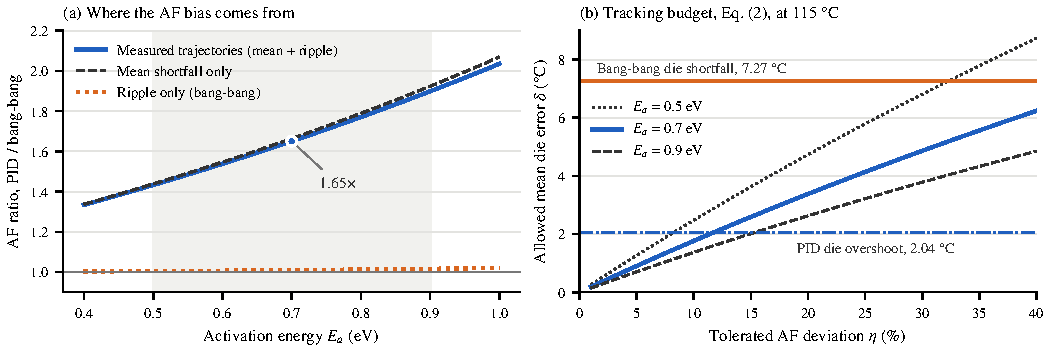
\includegraphics[width=\textwidth]{fig_stress.pdf}
\caption{Delivered stress in the \vDurPair-hour pair, from the measured die trajectories over each whole run. (a) PID-to-bang-bang ratio of delivered acceleration factor versus activation energy. The mean die-temperature shortfall alone reproduces the bias; thermostat ripple contributes \vRippleBB\% (shaded: commonly assumed $E_a$ range). (b) Allowed mean die-temperature error from Eq.~\eqref{eq:delta} versus tolerated AF deviation, with each bench's measured mean die error.}
\label{fig:stress}
\end{figure*}

The effect is not tied to one setpoint. At 100\degC{} oven air, the stock thermostat held a \vSdThermo\degC{} standard deviation, \vPtpThermo\degC{} peak-to-peak swing and \vEmaxThermo\degC{} maximum error over the last 30 minutes, against \vSdTuned, \vPtpTuned{} and \vEmaxTuned\degC{} under PID. These chamber-air figures are what the standards assess~\cite{jedec,mil}. The die-level data show what they leave out: the thermostat's air ripple was the visible symptom, but its mean die shortfall was the consequential error.

% ---------------------------------------------------------------
\section{Reversible noise: What the bench writes into the sensor}

The slack a sensor reports mixes a slow, permanent aging term with a fast, reversible PVT term. In the \vDurPair-hour pair, die temperature and voltage linearly explain \vRsqBB\% of slack variance under bang-bang and \vRsqPID\% under PID. A lower $R^2$ under PID is not lower fidelity: the controlled bench simply injects less environmental variance to explain. What matters downstream is the noise left after correction: the residual of the joint temperature--voltage fit is \vSigRawBB{} cnt under bang-bang and \vSigRawPID{} cnt under PID~\cite{sbcci26}, a \vSigRawRatio$\times$ higher noise floor for any AVS or alarm calibrated on the thermostatic bench~\cite{niemann}. The supply also oscillated more under bang-bang (\vVsdBB{} versus \vVsdPID\,mV standard deviation) despite compensation, because the die's leakage follows the thermal cycle. These short-term parameters are representative of long runs: the fast residual of the full \vDurBBlong-hour Week-1 log is \vBBlongSigRatio{} times that of its first day, and the long PID run's first-day fast residual is \vRCAfirstSigRatio{} times that of the whole run.

We tested two candidate mechanisms for the extra noise. Thermal lag between the XADC and the monitored path would make slack hysteretic in temperature; the measured heating-minus-cooling residual gap is \vHystBB\,cnt (\vHystPct\% of the residual), and a $dT/dt$ regressor lowers the residual by \vDtdtGainPct\%, so lag is not the mechanism. Nonlinear PVT coupling would leave information after linear correction. On the long PID run, temperature and voltage carry $I(S;T,V)=\vMIrawRCA$\,bits about the slack (\vHSRCA\,bits of entropy), and a linear correction removes \vRCAMIremoved\% of the short-term coupling; a per-bench comparison of what remains is inconclusive, because integer slack quantization alone reproduces it on the low-noise PID run. The thermostatic excess is therefore broadband variance, which no correction removes.

% ---------------------------------------------------------------
\begin{figure*}[!t]
\centering
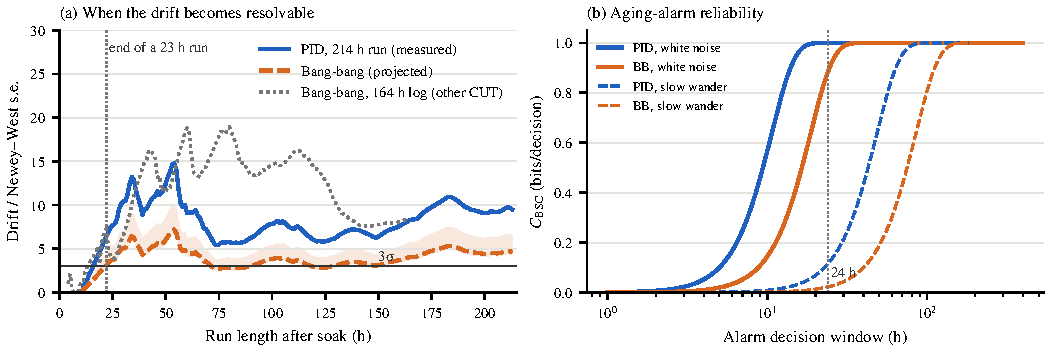
\includegraphics[width=\textwidth]{fig_detect.pdf}
\caption{Detectability. (a) Significance of the PVT-corrected slack drift versus run length (cumulative least-squares slope over Newey--West error with bandwidth up to 8\,h) on the \vDurRCA-hour PID run, and its projection to a thermostatic bench using the ratios measured on the \vDurPair-hour pair (band: aging law and $\tint$ ratio, Table~\ref{tab:tmin}). Dotted gray: the Week-1 thermostatic log, a different circuit on a then-unstressed device, whose early aging is faster. (b) Capacity of a threshold aging alarm, modeled as a binary symmetric channel, versus decision window: solid, white-noise bound; dashed, with the measured slow residual wander.}
\label{fig:detect}
\end{figure*}

\section{Detectability: When can a sensor see aging?}

\textbf{A drift is resolved, and it is sublinear.} After PVT correction, the \vDurRCA-hour residual drifts at \vBetaRCA\mcnth{} on average (95\% interval \vBetaLoRCA{} to \vBetaHiRCA), and its correlation with time strengthens from \vRCAcorrStRaw{} before correction to \vRCAcorrStCorr{} after it. The drift is not linear: it slows from \vRCAfirstHalf{} to \vRCAsecondHalf\mcnth{} between the two halves of the run, and a power law $t^{n}$ with $n=\vPowNRCA$ fits far better than a line ($\Delta\mathrm{BIC}=\vdBICblockRCA$ on 2-hour block means), consistent with bias-temperature instability. The total is \vRCAdriftCnt\,cnt, about \vRCAdriftPs\,ps of lost slack. We call it a drift, not aging, for two reasons: no logged channel can serve as an independent readout control, and the outer loop moved the oven setpoint \vRCAspChanges{} times (\vRCAspMin--\vRCAspMax\degC); \vSPjumpFrac\% of these moves coincide with a residual step beyond the 95th percentile at random times (5\% expected), a modest source of slow residual wander.

\textbf{The minimum burn-in time.} With $\sigma=\vSigRCA$\,cnt and $\tint=\vTauRCA$\,s for the fast residual and the average $\beta$, Eq.~\eqref{eq:tmin} gives $\Tmin=\vTminBound$\,h. The residual does not decorrelate within $\tint$, however: its long-run variance keeps growing with averaging time, \vRCAlrvGrowth-fold from 15-minute to 8-hour blocks, and the 8-hour value raises $\Tmin$ to \vTminLrv\,h. Conversely, because the drift is fastest early, the cumulative slope crosses 3$\sigma$ for good after \vTminSeq\,h [Figure~\ref{fig:detect}(a)], a descriptive time rather than a stopping rule. Table~\ref{tab:tmin} collects the three; none is wrong, they answer the question under different assumptions about noise and aging law. The same holds for the 23-hour runs: SBCCI~2026 found nonzero late-window slopes in both at 95\% confidence~\cite{sbcci26}, but whether such a slope is aging cannot be decided within a day, which is what the long run settles.

\begin{table}[!t]
\centering
\caption{Burn-in duration (h) to resolve the drift at 3$\sigma$, PID long run and projected thermostatic bench (range: aging law and $\tau_{\mathrm{int}}$ ratio); bottom row: alarm window for 0.99\,bits.}
\label{tab:tmin}
\scriptsize
\setlength{\tabcolsep}{2.0pt}
\begin{tabular}{@{}l l r l@{}}
\toprule
Method & Noise / drift model & PID & Thermostatic \\
\midrule
Eq.~\eqref{eq:tmin} & white, mean rate & \vTminBound & \vTminBBBound{} (\vTminBBBoundLo--\vTminBBBoundHi) \\
Eq.~\eqref{eq:tmin}, long-run var. & 8\,h wander, mean rate & \vTminLrv & \vTminBBLrv{} (\vTminBBLrvLo--\vTminBBLrvHi) \\
Sequential test & measured, as observed & \vTminSeq & \vTminBBSeq{} (\vTminBBSeqLo--\vTminBBSeqHi) \\
Week-1 log, inverters & measured, unstressed device & -- & \vTminSeqBBlong{} (measured) \\
\midrule
Alarm, $C\ge0.99$ & white / 8\,h wander & \vWpidBound{} / \vWpidLrv & \vWbbBound{} / \vWbbLrv \\
\bottomrule
\end{tabular}
\end{table}

\textbf{The bench penalty.} Eq.~\eqref{eq:tmin} shows how the bench enters: through the noise $\sigma$ and decorrelation $\tint$ it injects, and through the stress it delivers, which sets $\beta$. On the paired runs the thermostatic bench raises $\sigma$ by \vSigRawRatio$\times$. Compared at a common sampling interval, both inverter-chain residuals are close to white ($\tint$ of \vTauBBs{} and \vTauPIDs\,s), unlike the adder's. The stress enters through the aging law. If drift rate scales with delivered AF, the stress penalty is $\vAFratio^{2/3}=\vPenStress\times$; if drift follows the fitted power law in equivalent time, $(AF\,t)^{\vNLaw}$, it is only \vPenStressPow$\times$. With the noise penalty of $\vSigRawRatio^{2/3}=\vPenNoiseSigOnly\times$, a thermostatic bench would need a projected \vPenLow--\vPenMid$\times$ longer, or \vPenHigh$\times$ with the measured $\tint$ ratio (Table~\ref{tab:tmin}); after \vDurPairPost\,h it would sit at \vSeqZbb$\sigma$, on the threshold, where the PID run already stood at \vSeqZpid$\sigma$. This projection carries a noise ratio measured on the inverter chain to the adder, an assumption these data cannot test. The thermostatic Week-1 log itself resolved its drift after \vTminSeqBBlong\,h [Figure~\ref{fig:detect}(a)]: on an unstressed device, early aging is fast enough to show through the thermostat's noise. Detection time depends on the device's aging state as much as on the bench.

\textbf{Alarm reliability.} SLM functions consume decisions, not slopes~\cite{kashyap}. Under white noise, a 24-hour alarm on the PID run errs with probability \vPerrPidBound\% (\vCpidBound\,bits per decision), the projected thermostatic one with \vPerrBbBound\% (\vCbbBound); with the measured slow wander these become \vPerrPidLrv\% and \vPerrBbLrv\% [Figure~\ref{fig:detect}(b); Table~\ref{tab:tmin}]. An alarm window chosen on one bench is mis-set on the other, adding bench-induced missed and false alarms to those a sensor's own calibration drift already causes~\cite{anik}.

\textbf{From detectability to failure.} Detectability does not say how far the circuit is from failing. Our sensor work validated a flip-flop failure catcher at the end of the monitored path that records a real timing violation at the sensor-reported failure point, within clock-jitter margin~\cite{sbcci25}. Sensor slack thus has a physical zero, and a detected drift becomes a distance to failure under stress. We do not extrapolate a lifetime from one board and one operating point.

% ---------------------------------------------------------------
\section{What labs should report}

The standards behave as designed: they bound the chamber, and the thermostatic bench's air ripple would be flagged by them. What they do not bound is the stress and noise reaching a powered die, which is what a critical-path sensor samples. For sensor-instrumented burn-in we propose the five-item report of Table~\ref{tab:checklist}. Each item is computable from a standard 1-Hz log, and together they let a reader judge whether a published aging curve reflects the device or the bench. The two items most often missing in FPGA aging studies~\cite{valdes,sobas}, die-level mean temperature and $\Tmin$, are also the two that change the conclusions most in our data.

\begin{table}[!t]
\centering
\caption{Proposed reporting checklist for sensor-instrumented burn-in, with values from this study.}
\label{tab:checklist}
\footnotesize
\setlength{\tabcolsep}{2.5pt}
\begin{tabular}{@{}p{27mm} p{56mm}@{}}
\toprule
Item & This study \\
\midrule
1. Die trajectory: mean, std.\ dev., error vs.\ target & BB \vTBB\,\textdegree C, \vTsdBB, \vTerrBB; PID \vTPID\,\textdegree C, \vTsdPID, $+$\vTerrPID \\
2. Delivered $\langle AF\rangle$ with $E_a$ range & BB \vAFBB, PID \vAFPID{} at 0.7\,eV; ratio about \vAFratioLoOne--\vAFratioHiOne \\
3. Post-PVT residual $\sigma$ & BB \vSigRawBB, PID \vSigRawPID\,cnt (23\,h); \vSigRCA\,cnt (\vDurRCA\,h, fast) \\
4. $\tint$; long-run variance vs.\ averaging time & \vTauRCA\,s; \vRCAlrvGrowth-fold growth, 15\,min to 8\,h \\
5. $\Tmin$ vs.\ run length, with method & Table~\ref{tab:tmin} \\
\bottomrule
\end{tabular}
\end{table}

\textbf{Limitations.} All data come from one 28\,nm board, so bench effects are established within one device, not as population statistics. The two comparisons use different monitored circuits, and the paired runs were separate campaigns at different points in the device's stress history. The thermostatic detectability figures are projections that bracket the aging law and transfer a noise ratio between circuits. No logged channel isolates readout drift. Because the stress is overstress, mechanisms beyond field-representative aging may contribute; the findings concern the bench, not the device's lifetime. Statements about JEDEC and MIL-STD conditions~\cite{jedec,mil} are interpretive and do not claim chamber certification.

% ---------------------------------------------------------------
% [SLOT: 16 nm FinFET transfer -- Artix UltraScale+ runs; go/no-go 2026-11-15]
% Keep commented out. The contingency version must compile and read complete
% without it. If enabled: one paragraph + at most one figure/table; add its
% numbers to analysis/ (new campaign key in dtlib.CAMPAIGNS) and to values.tex;
% re-run analysis/wordcount.py (budget headroom is printed there).
% \section{Transfer to a 16\,nm FinFET FPGA}
% ...
% ---------------------------------------------------------------

% Closing (CEDA: 1-2 paragraphs, lessons learned and future rather than a summary)
\section{Conclusion}

The question this article posed has a measured answer on the PID bench, a detection time of \vTminSeq--\vTminLrv\,h depending on the noise model and the aging law, and a projected one for the thermostatic bench, \vPenLow--\vPenHigh$\times$ longer. The lesson for anyone validating an on-chip sensor under burn-in is that the bench belongs in the measurement chain. Its dominant error was the mean die temperature, which chamber-level specifications cannot reveal, rather than the ripple they police, and it reached the sensor twice: as a \vAFratio$\times$ shortfall in delivered stress and as a \vSigRawRatio$\times$ higher residual noise floor. Because detection time also depends on the device's aging state, the checklist asks for the method behind any reported $\Tmin$, not only its value.

Three extensions follow directly. A matched-duration thermostatic campaign on the same circuit would replace the projection with a measurement; multi-device replication would turn within-device bench effects into population statistics; and a 16\,nm FinFET platform, where published drifts are below 0.1\% over 1,000 hours even at elevated stress~\cite{sobas}, will test whether the bench-set detection floor tightens as expected. Sensor-validated burn-in now feeds SLM, so these benches should be reported with the same care as the sensors they validate.

% ---------------------------------------------------------------
\renewcommand{\refname}{References}\begin{thebibliography}{12}
\footnotesize
% TODO(authors): inclusive pages for Kashyap IRPS 2021 (D&T requires them); DOI verified
\bibitem{kashyap} R.~Kashyap, ``Silicon lifecycle management (SLM) with in-chip monitoring,'' in \emph{Proc. IEEE Int. Rel. Phys. Symp. (IRPS)}, 2021, doi: 10.1109/IRPS46558.2021.9405187.
\bibitem{niemann} C.~Niemann, M.~Ali, O.~U.~Shah, J.~Heller, and D.~Timmermann, ``Sensor based adaptive voltage scaling on FPGAs: Calibration and parametrization,'' \emph{Integration}, vol.~75, pp.~30--39, 2020, doi: 10.1016/j.vlsi.2020.05.006.
\bibitem{valdes} M.~Vald\'es-Pe\~na \emph{et al.}, ``Design and validation of configurable online aging sensors in nanometer-scale FPGAs,'' \emph{IEEE Trans. Nanotechnol.}, vol.~12, no.~4, pp.~508--517, 2013, doi: 10.1109/TNANO.2013.2253795.
\bibitem{jedec} \emph{Temperature, Bias, and Operating Life}, JEDEC Standard JESD22-A108G, 2022.
\bibitem{mil} \emph{Test Method Standard: Microcircuits, Method 1015: Burn-In Test}, MIL-STD-883, U.S. Department of Defense, 2016.
\bibitem{vassighi} A.~Vassighi, O.~Semenov, M.~Sachdev, A.~Keshavarzi, and C.~Hawkins, ``CMOS IC technology scaling and its impact on burn-in,'' \emph{IEEE Trans. Device Mater. Rel.}, vol.~4, no.~2, pp.~208--221, 2004, doi: 10.1109/TDMR.2004.826591.
\bibitem{semenov} O.~Semenov, A.~Vassighi, M.~Sachdev, A.~Keshavarzi, and C.~F.~Hawkins, ``Effect of CMOS technology scaling on thermal management during burn-in,'' \emph{IEEE Trans. Semicond. Manuf.}, vol.~16, no.~4, pp.~686--695, 2003, doi: 10.1109/TSM.2003.818985.
\bibitem{anik} M.~T.~H.~Anik, S.~Guilley, J.-L.~Danger, and N.~Karimi, ``On the effect of aging on digital sensors,'' in \emph{Proc. 33rd Int. Conf. VLSI Design (VLSID)}, 2020, pp.~189--194, doi: 10.1109/VLSID49098.2020.00050.
\bibitem{sbcci26} D.~Alencar \emph{et al.}, ``Quantifying the effect of burn-in thermal control on delivered acceleration factor and on-chip slack-sensor fidelity in an FPGA target,'' in \emph{Proc. 39th Symp. Integr. Circuits Syst. Design (SBCCI)}, 2026, to be published.
\bibitem{sbcci25} L.~Nogueira \emph{et al.}, ``Auto-tuning aging sensor validated under burn-in, temperature, and voltage variations,'' in \emph{Proc. 38th Symp. Integr. Circuits Syst. Design (SBCCI)}, 2025, pp.~1--5.
\bibitem{simc} S.~Skogestad, ``Simple analytic rules for model reduction and PID controller tuning,'' \emph{J. Process Control}, vol.~13, no.~4, pp.~291--309, 2003.
\bibitem{sobas} J.~Sobas, T.-B.~Airimitoaie, and F.~Marc, ``Development of a high accuracy and stability test bench for ageing measurement of 16\,nm FinFETs based FPGA,'' \emph{Microelectron. Rel.}, vol.~138, 2022, Art. no.~114698, doi: 10.1016/j.microrel.2022.114698.
\end{thebibliography}

% ---------------------------------------------------------------
% Biographies (CEDA: position, highest degree, discipline, institution, <= 3 interests, memberships, e-mail)
\section*{Author Biographies}
\footnotesize
\noindent\textbf{Danilo Alencar} is a master's student in teleinformatics engineering at the Universidade Federal do Cear\'a (UFC), Fortaleza, Brazil, and a researcher at the Laboratory of Electronic Systems and Circuits (LESC). His research interests include FPGA reliability, aging instrumentation, and silicon lifecycle management. Alencar has a BSc in computer engineering from UFC. Contact him at danilo.alencar@lesc.ufc.br.

\smallskip\noindent\textbf{Lucas Nogueira} is with LESC, UFC, Fortaleza, Brazil. His research interests include on-chip aging sensors and FPGA delay monitoring. Contact him at lucas.nogueira@lesc.ufc.br.

% TODO(authors): complete co-author bios per CEDA (position, highest degree + discipline + institution, <=3 interests, memberships, e-mail)
\smallskip\noindent\textbf{Alisson Barros}, \textbf{Arthur Pamplona}, and \textbf{Andre Grangeiro} are with LESC, UFC, Fortaleza, Brazil. Their research interests include FPGA test platforms and reliability instrumentation.

\smallskip\noindent\textbf{Jarbas Silveira} is a professor at UFC, Fortaleza, Brazil, and leads research at LESC. His research interests include integrated-circuit design, test, and reliability. Contact him at jarbas@lesc.ufc.br.

\smallskip\noindent\textbf{Fabian Vargas} is with IHP -- Leibniz Institute for High Performance Microelectronics, Frankfurt (Oder), Germany. His research interests include on-chip sensors, design for reliability, and silicon lifecycle management. Contact him at vargas@ihp-microelectronics.com.

\medskip\noindent Direct questions and comments about this article to Danilo Alencar, Laboratory of Electronic Systems and Circuits (LESC), Universidade Federal do Cear\'a, Fortaleza, CE, Brazil; danilo.alencar@lesc.ufc.br.

\end{document}
